\documentclass[
  twoside,
  11pt, a4paper,
  footinclude=true,
  headinclude=true,
  cleardoublepage=empty
]{scrreprt}

\usepackage{lipsum}
\usepackage[ngerman,english]{babel}
\usepackage{amsmath}
\usepackage{amsthm}
\usepackage{graphicx}
\usepackage{listings}
\usepackage{lmodern}
\usepackage{float}
\usepackage{csquotes}
\usepackage{sidecap}
\usepackage{acronym}
\usepackage{setspace}
\usepackage{url}
\usepackage[T1]{fontenc}
\usepackage[utf8]{inputenc}
\graphicspath{ {images/} }

\begin{document}

\begin{titlepage}
    \begin{center}
        \Huge
        \textbf{Feasibility Study of Real Time Path Tracing}
        
        \vspace{0.5cm}

        \LARGE
        \textit{Or:} How Much Noise Is Too Much?
        
        \vspace{1.5cm}
        
        \textbf{Sven-Hendrik Haase}
        
        \vfill
        
        A thesis presented for the degree of\\
        \emph{Bachelor of Computer Science}
        
        \vspace{0.8cm}
        
        
\includegraphics[width=0.4\textwidth]{frontbackmatter/logo_uhh.jpg}
        
        % I was not allowed to use the old logo :( But I have much like it so I'm
        % keeping this here.
        %
\includegraphics[width=0.4\textwidth]{frontbackmatter/uni-siegel.png}
        
        \Large
        Department of Informatics\\
        University of Hamburg\\
        Germany\\
        2015-20-08

        \vspace{0.8cm}

        \large
        Primary Supervisor: Prof. Dr. rer. nat. Leonie \textsc{Dreschler-Fischer}\\
        Secondary Supervisor: Prof. Dr. Thomas \textsc{Ludwig}
        
    \end{center}
\end{titlepage}


\chapter*{Abstract}
\onehalfspace
This study aims to investigate the viability of a physically-based technique called
\textbf{path tracing} in lieu of or in corporation with classical techniques in interactive media such as video
games and visual effects tools.

Real time path tracing has been prohibitively expensive in regards to computational
complexity. However, modern \acs{gpu}s and even \acs{cpu}s have finally gotten fast enough for real time path
tracing to become a viable alternative to traditional real time approaches to rendering.  Based on
that assumption, this thesis presents the idea, algorithm and complexity behind path tracing in the
first part and extrapolates feasibility and suitability of real time path tracing on consumer
hardware according to the current state of technology and trends in the second part.

As part of the research, the author has implemented a path tracing 3D engine in modern C++ in order
to empirically test the assumptions made in this thesis. The study found path tracing
to be a viable rendering technique for average commodity hardware in approximately 4 years.
\singlespace

\chapter*{Acknowledgments}
\doublespacing
I would like to express my sincere gratitude to the teachers throughout school and university for
the knowledge they've passed on.

I thank my friends for the laughs, horrible mistakes and awesome successes we shared with
one another.

Furthermore, none of this would have been possible without the incredible efforts and love of my
parents who have supported me throughout the years and enabled me to live a carefree life until I
was ready to fend for myself.

Lastly, but certainly not least, I would like to declare my gratefulness to Alisa, whose endless love
has given my life a new meaning.

\singlespace

\clearpage
\vspace*{\fill}
\thispagestyle{empty} % suppress showing of page number
\begin{quotation}
    \em
    We all make choices in life, but in the end, our choices make us.

    \medskip
    \raggedleft
    Andrew Ryan
\end{quotation}
\vspace*{\fill}

\tableofcontents

\chapter*{Acronyms}
\begin{acronym}
    \acro{aabb}[AABB]{axis-aligned bounding box}
    \acro{ao}[AO]{ambient occlusion}
    \acro{brdf}[BRDF]{bidirectional reflection distribution function}
    \acro{bsp}[BSP]{binary space partitioning}
    \acro{cpu}[CPU]{central processing unit}
    \acro{csg}[CSG]{constructive solid geometry}
    \acro{fps}[FPS]{frames per second}
    \acro{gi}[GI]{global illumination}
    \acro{gpu}[GPU]{graphics processing unit}
    \acro{hdr}[HDR]{high dynamic range}
    \acro{mlt}[MLT]{Metropolis light transport}
    \acro{pbr}[PBR]{physically based rendering}
    \acro{rt}[RT]{real time}
    \acro{rgb}[RGB]{red-green-blue}
    \acro{simd}[SIMD]{single instruction multiple data}
    \acro{spp}[SPP]{samples per pixel}
    \acro{ssao}[SSAO]{screen-space ambient occlusion}
\end{acronym}

\chapter{Introduction}
As part of the quest for ever-improving game graphics, researchers, graphics hardware developers
and video game developers alike have been coming up with more and more convoluted and technically
challenging ways of improving the graphics in interactive media such as games and visualizations in
order to give users a deeper sense of immersion or to provide special effects artists with faster
feedback.

While rendering techniques are currently shifting from the traditional fixed pipeline approach
towards the new, fully programmable approach that lets developers implement deferred renderers that
can more closely mimic reality by using multiple combined shading and lighting algorithms and
rendering the scene multiple times for different buffers, the fundamental concept of
rasterization-based rendering has largely remained the same.

The real world photon-collecting approach that actual cameras use has so far not been adopted for
interactive media by the industry in any capacity because the computational cost has historically
been prohibitively expensive. It is, however, used extensively (and has been in use since decades)
for offline, non-interactive rendering of computer-generated movies and visualizations of
scientific simulations.

This study assumes that the next logical step for the industry will be to adopt this method for
real time media as well. For the purpose of this thesis, a renderer is considered
\textit{real time} when it manages to render a frame within \(16.67ms\) since that equals 60
\ac{fps} which is
the current de-facto standard refresh rate for most available computer screens. Conversely, a
renderer is called \textit{offline} when it is not designed for interactive rendering which usually
means that it will renderer an image or a batch of images over the course of a few days. The
differences of real time and offline path tracing renderers will be explained in the next chapter.

\section{Motivation}
Real time path tracing (and physically based rendering in general) offers many
benefits over traditional real time rendering methods such as better visuals
and simpler implementation but also allows for completely new types of graphics
such as realistic caustics \cite{wiki:caustics} and even light dispersion
\cite{wiki:dispersion} (using a prism, for instance) since path tracers might simulate wavelengths
instead of plain \ac{rgb} colors. Modern video games tend
to rely on a growing number of tricks to keep them visually appealing as the
consumer grows more demanding. They're called \textit{tricks} in this study
because they merely trick the beholder into seeing something that appears to be
physically accurate when it is, in fact, not the result of a physically-based
calculation and as such this study aims to keep tricks and emergent phenomena
separated by language. Some notable tricks include \ac{ssao}
\cite{wiki:ssao}, motion blur \cite{wiki:motion-blur}, lens flares
\cite{wiki:lens-flare}, chromatic aberration \cite{wiki:chromatic-aberration},
depth of field \cite{wiki:depth-of-field} and light mapping \cite{wiki:lightmap}.

\chapter{Real Time Path Tracing Explained}
This chapter will explain the concepts, mathematics and algorithms behind path tracing, how real
time path tracing differs from offline path tracing and what the difference in speed means for
quality. It will also explain how path tracing differs from rasterization and other global
illumination techniques.

\section{Theoretical Basis}
This explanation will
\lipsum[1]

\section{Path Tracing in Comparison to Other Techniques}

\subsection{Comparison to Rasterization}

\subsection{Comparison to Other Algorithms}

\section{History of Path Tracing}
As with so many things in computer science and science in general, the modern idea of physically
based rendering using path tracing builds upon many important past discoveries and algorithms
such as ray tracing and ray casting.
Arthur Appel is generally credited as being the father of
\emph{ray casting} as he was the first to describe the algorithm in a 1968 paper
\cite{inproceedings:raycasting}.

Ray casting is an important idea needed for \emph{ray tracing} which was
first published in a paper in 1980 by Turner Whitted \cite{article:raytracing}.

\begin{figure}[h]
    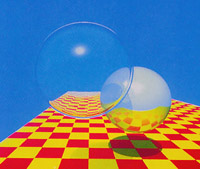
\includegraphics{early-raytracing-whitted}
    \centering
    \caption{Turner Whitted's original 1980 \cite{article:raytracing} image showing off the usage of ray tracing for
    reflection, refraction and shadows.}
    \label{fig:early-raytracing-whitted}
\end{figure}

Building upon ray tracing, an improved algorithm was published in 1986 by James T. Kajiya which used ray tracing
combined with a Monte Carlo algorithm in order to create a new algorithm that was called \emph{Monte
Carlo ray tracing} \cite{inproceedings:pathtracing}. Nowadays, Monte Carlo ray tracing is better
known as \emph{path tracing}.

It took another decade for path tracing to become the
physically based rendering approach that it is known for today. In 1996, Eric Lafortune improved
the algorithm by suggesting the usage of bidirectional path tracing \cite{techreport:pbr} and
finally the Metropolis light transport was suggested in 1997 by Eric Veach and Leonidas J. Guibas \cite{inproceedings:metropolis} to
improve performance in complex scenes.

This was the last notable improvement to the algorithm,
though many micro optimizations have since been published. All of these achievements and
improvements are generally collapsed into the term \emph{path tracing} since they do not diverge
from the general algorithm but instead improve upon it.

It took longer still for the industry to become interested in path tracing. The early interest in
ray tracing was of mostly academical and recreational nature. One of the most notable creations of
the early days of ray tracing is The Juggler created and published by Eric Graham in 1986
\cite{site:juggler} on an Amiga 1000. It was a pre-rendered animation using ray tracing. Eric Graham
stated that it took the Amiga 1 hour to render each frame \cite{site:juggler}.

\begin{figure}[H]
    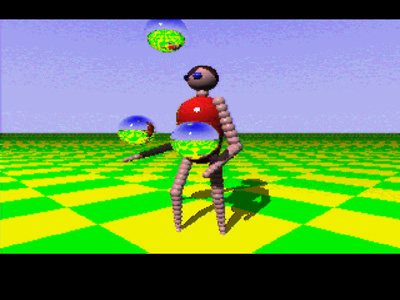
\includegraphics[scale=0.5]{amiga-juggler}
    \centering
    \caption{Eric Graham's Juggler}
    \label{fig:amiga-juggler}
\end{figure}

While the animation seems very primitive compared to the animations of today, it was exceptional at
the time. Ernie Wright's statement about The Juggler provides some contemporary context:
\blockquote[\cite{site:juggler}]{Turner Whitted's paper (1980) is widely regarded as the first modern
description of ray tracing methods in computer graphics. This paper's famous image of balls floating
above a checkerboard floor took 74 minutes to render on a DEC VAX 11/780 mainframe, a \$400,000
computer. The Juggler would appear a mere six years later, created and displayed on a \$2000 Amiga.}

The first feature-length computer-animated film,
\textit{Toy Story}, released in 1995 \cite{wiki:toy-story}, is sometimes miscredited as being the
first film using a ray tracing-like algorithm. However, it actually used traditional scanline
rendering. The first feature-length film using ray tracing, \textit{Cars}, was released much later,
in 2006 \cite{wiki:cars} \cite{inproceedings:cars} and started a wave of interest in the movie industry.

\section{Current State of Technology}
lol
\lipsum[1]

\chapter{Research}
\lipsum[1]

\section{Results}
\lipsum[1]

\section{Evaluation}
\lipsum[1]

\chapter{Conclusion}
\lipsum[1]

\section{Outlook}
\lipsum[1]

\listoffigures
 
\listoftables

\bibliographystyle{unsrt}
\bibliography{main}
    
\end{document}
